\documentclass[tikz,border=5mm]{standalone}
\usepackage{tikz}
\usetikzlibrary{shapes, arrows, positioning, calc}

\begin{document}
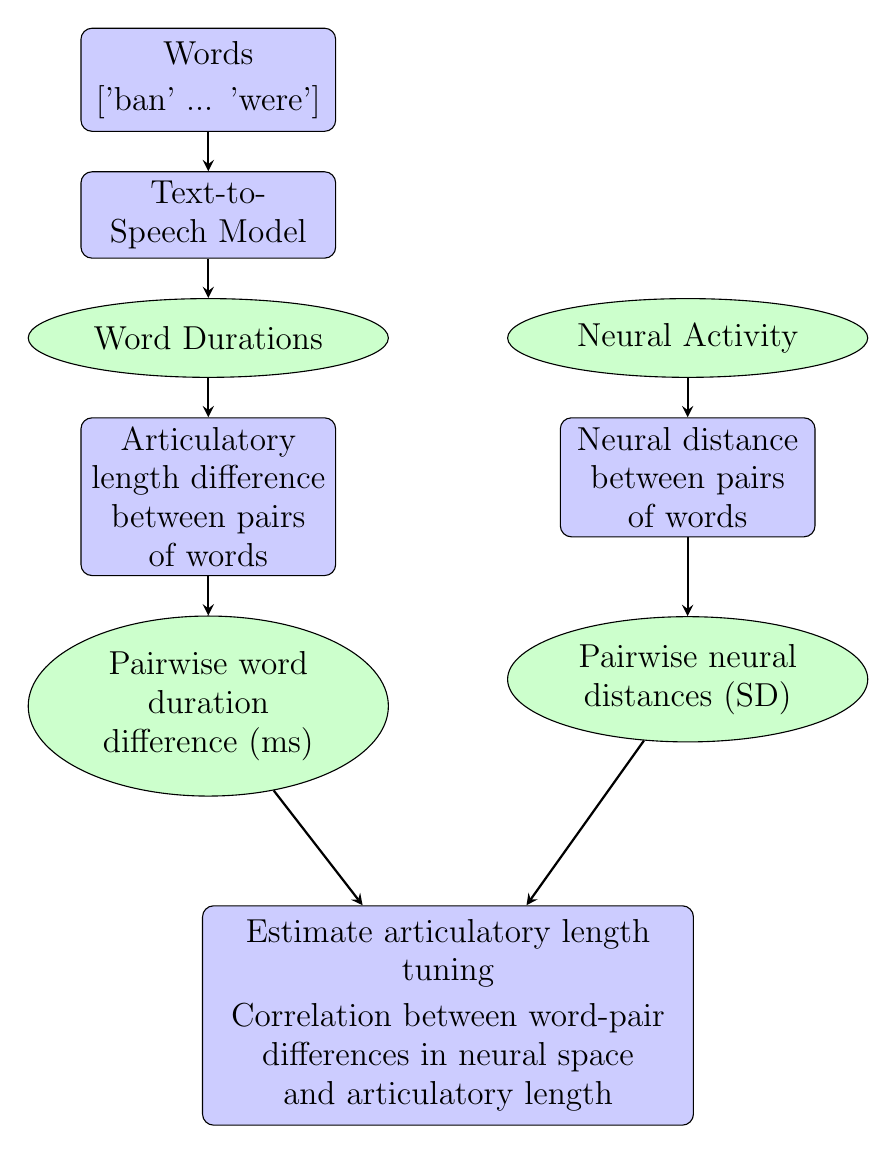
\begin{tikzpicture}[node distance=1.8cm, auto,
    % Define node styles that set text width and font size.
    process/.style={
      rectangle, rounded corners, minimum height=1cm, 
      text centered, draw=black, fill=blue!20, 
      text width=3cm, align=center, font=\large
    },
    data/.style={
      ellipse, minimum height=1cm, 
      text centered, draw=black, fill=green!20, 
      text width=3cm, align=center, font=\large
    },
    arrow/.style={thick,->,>=stealth}
]

% Node 1: Input Text with tabular content (fixed width) 
\node [process] (inputtext) {%
  \begin{tabular}{@{}p{3cm}@{}}
    \centering \large Words\\[0.5ex]
    {['ban' ... 'were']}
  \end{tabular}
};

% Node 2: TTS Model
\node [process, below=0.5cm of inputtext] (tts) {Text-to-Speech Model};

% Node 5: Word Durations (data node)
\node [data, below=0.5cm of tts] (durations) {Word Durations};

% Node 6: Articulatory length difference between pairs of words
\node [process, below=0.5cm of durations] (articulatorDistance) {Articulatory length difference\\between pairs of words};

% Node 7: Pairwise word duration difference (data node)
\node [data, below=0.5cm of articulatorDistance] (pairwiseArticulatoryDist) {Pairwise word duration difference (ms)};

% Node 8: Neural Activity (data node) placed to the right of the durations node
\node [data, right=1.5cm of durations] (neural) {Neural Activity};

% Node 9: Neural distance between pairs of words (process node)
\node [process, below=0.5cm of neural] (neuralDistance) {Neural distance between pairs of words};

% Node 10: Pairwise neural distances (data node)
\node [data, below=1cm of neuralDistance] (pairwiseNeuralDist) {Pairwise neural distances (SD)};

% Node 11: Analysis node
% It is placed 2.7cm below the midpoint between pairwiseArticulatoryDist and pairwiseNeuralDist
% and given a larger text width (6cm) and minimum height to accommodate more text.
\node [process, 
       below=2.7cm of $(pairwiseArticulatoryDist)!0.5!(pairwiseNeuralDist)$, 
       text width=6cm,
       minimum height=2cm] (analysis) {%
  \begin{tabular}{@{}p{6cm}@{}}
    \centering \large Estimate articulatory length tuning\\[0.5ex]
    Correlation between word-pair differences in neural space\\ and articulatory length
  \end{tabular}
};

% Draw arrows connecting the nodes
\draw [arrow] (inputtext) -- (tts);
\draw [arrow] (tts) -- (durations);
\draw [arrow] (durations) -- (articulatorDistance);
\draw [arrow] (articulatorDistance) -- (pairwiseArticulatoryDist);
\draw [arrow] (pairwiseArticulatoryDist) -- (analysis);
\draw [arrow] (neural) -- (neuralDistance);
\draw [arrow] (neuralDistance) -- (pairwiseNeuralDist);
\draw [arrow] (pairwiseNeuralDist) -- (analysis);

\end{tikzpicture}
\end{document}
